\documentclass{beamer}

\usepackage{hyperref}
\usepackage{graphicx}
\usepackage{tikz}
\usetikzlibrary{calc}

\newcommand{\NH}{\text{NH}}
\newcommand{\RG}{\text{RG}}

\title{Measuring the Price of Anarchy in Critical Care Unit Interactions}
\author{Vincent Knight and Izabella Komenda}
\date{2014-07-25}

\setbeamertemplate{navigation symbols}{}

\begin{document}

\frame{
\begin{center}
\href{https://plus.google.com/+VincentKnight/posts}{+Vincent.Knight}\\
\href{https://twitter.com/drvinceknight}{@drvinceknight}\\
\href{http://drvinceknight.github.io/Talks/}{drvinceknight.github.io/Talks}\\
\vspace{1cm}
\href{https://twitter.com/IzabelaKomenda}{@IzabelaKomenda}\\
Professor Jeff Griffiths
\end{center}
}

\frame{
    \Huge
    \[
        \begin{pmatrix}
        (2,2)&(5,0)\\
        (0,5)&(4,4)
        \end{pmatrix}
    \]
}

\frame{
    \begin{center}
        \includegraphics[width=.8\textwidth]{./Images/PoA_Healthcare.pdf}
    \end{center}
}

\frame{
    \begin{center}
        {\Huge What about the controllers?}\\
        \vspace{1cm}
    \end{center}
        \pause
        S. Deo and I. Gurvich. \textbf{Centralized vs. Decentralized Ambulance Diversion: A Network Perspective.} \textit{Management Science}, 57(7):1300–1319, May 2011.
}

\frame{
    \begin{center}
        \includegraphics[width=.8\textwidth]{./Images/RG_state_dependent_model.jpg}
    \end{center}
    \pause
    \textbf{Mathematical modelling of patient flows to predict critical care capacity required following the merger of two District General Hospitals into one.}, \textit{Submitted to Anaesthesia}
}

\frame{
\begin{center}
    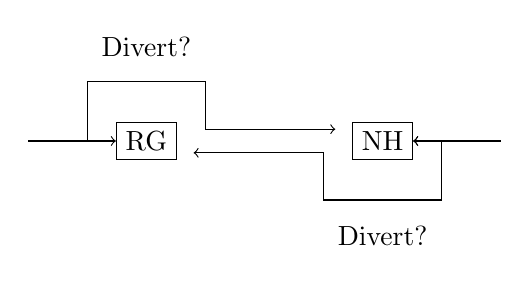
\begin{tikzpicture}[scale=1.5]
        \node (A) at (0,0) [draw] {RG};
        \node (B) at (2,0) [draw] {NH};
        \draw [->] (-1,0) -- (A);
        \draw [->] (3,0) -- (B);
        \draw [->] (-1,0) -- ($(A)+(-.5,0)$) -- ($(A)+(-.5,.5)$) -- ($(A)+(.5,.5)$) -- ($(A)+(.5,.1)$) -- ($(B)+(-.4,.1)$);
        \draw [->] (3,0) -- ($(B)+(.5,0)$) -- ($(B)+(.5,-.5)$) -- ($(B)+(-.5,-.5)$) -- ($(B)+(-.5,-.1)$) -- ($(A)+(.4,-.1)$);
        \draw [->] (3,0) -- (B);
        \node at ($(A) + (0,.8)$) {Divert?};
        \node at ($(B) + (0,-.8)$) {Divert?};
    \end{tikzpicture}
\end{center}
}

\frame{
\begin{center}
    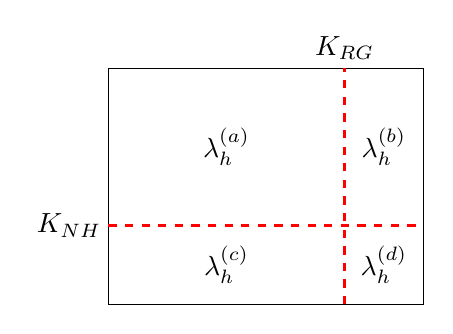
\begin{tikzpicture}
        \draw  (0,0) rectangle (4,3);
        \draw [dashed, red, thick] (0,1) -- (4,1);
        \draw [dashed, red, thick] (3,0) -- (3,3);
        \node at (-.5,1) {$K_{\NH}$};
        \node at (3,3.25) {$K_{\RG}$};
        \node at (1.5,2) {$\lambda_{h}^{(a)}$};
        \node at (3.5,2) {$\lambda_{h}^{(b)}$};
        \node at (1.5,.5) {$\lambda_{h}^{(c)}$};
        \node at (3.5,.5) {$\lambda_{h}^{(d)}$};
    \end{tikzpicture}
\end{center}
}

\frame{
\begin{center}
    \only<1>{
        \input{mc.tex}
    }
    \only<2>{
    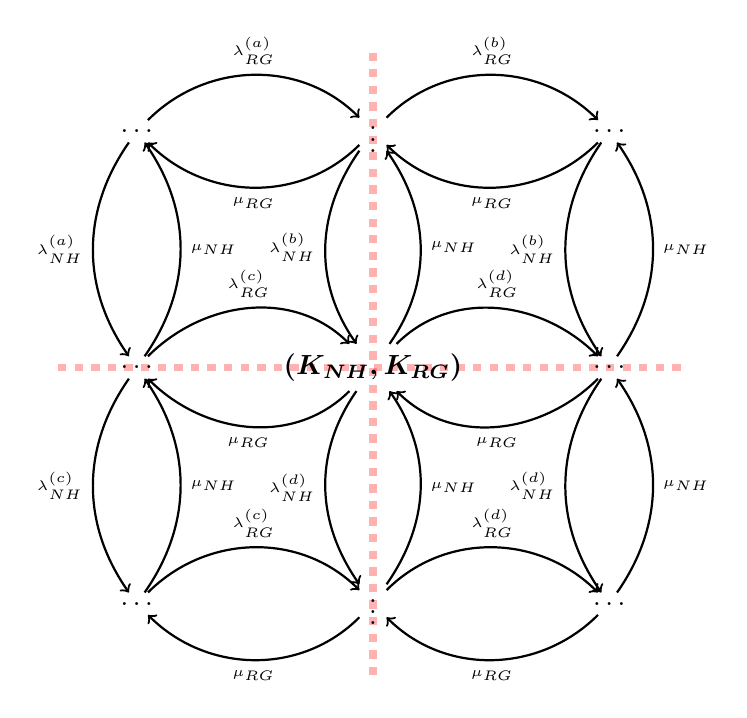
\begin{tikzpicture}[scale=1, every node/.style={scale=1}]
    % -----------------------------------------------
    % Boundaries ------------------------------------
    % -----------------------------------------------
    \draw [dashed, line width=1mm, red, opacity=.3] (2,-3) -- (10,-3);
    \draw [dashed, line width=1mm, red, opacity=.3] (6,1) -- (6,-7);
    %\tikzstyle{state}=[ellipse, draw, fill=blue!10, minimum width=2cm];
    %\tikzstyle{state}=[rectangle, draw, fill=blue!10, minimum width=2cm];
    \tikzstyle{state}=[minimum width=2cm, font=\boldmath];

    % -----------------------------------------------
    % Fourth row--------------------------------------
    % -----------------------------------------------
    \node (ellipsisd1) at ($(0,0) + (3,0)$) {$\dots$};
    \node(dk) at ($(ellipsisd1) + (3,0)$) {$\vdots$};
    \node (ellipsisd2) at ($(dk) + (3,0)$) {$\dots$};
    % Transitions -----------------------------------
    % On Row:
    \draw (ellipsisd1) edge[out=45,in=135,->,thick] node [above] {\tiny$\lambda_{\RG}^{(a)}$} (dk);
    \draw (ellipsisd1) edge[out=-45,in=-135,<-,thick] node [below] {\tiny$\mu_{\RG}$} (dk);

    \draw (dk) edge[out=45,in=135,->,thick] node [above] {\tiny$\lambda_{\RG}^{(b)}$} (ellipsisd2);
    \draw (dk) edge[out=-45,in=-135,<-,thick] node [below] {\tiny$\mu_{\RG}$} (ellipsisd2);

    % -----------------------------------------------
    % Fifth row--------------------------------------
    % -----------------------------------------------
    \node (ellipsise1) at ($(0,-3) + (3,0)$) {$\dots$};
    \node(ek) [state] at ($(ellipsise1) + (3,0)$) {$(K_{\NH},K_{\RG})$};
    \node (ellipsise2) at ($(ek) + (3,0)$) {$\dots$};
    % Transitions -----------------------------------
    % On Row:
    \draw (ellipsise1) edge[out=45,in=135,->,thick] node [above] {\tiny$\lambda_{\RG}^{(c)}$} (ek);
    \draw (ellipsise1) edge[out=-45,in=-135,<-,thick] node [below] {\tiny$\mu_{\RG}$} (ek);

    \draw (ek) edge[out=45,in=135,->,thick] node [above] {\tiny$\lambda_{\RG}^{(d)}$} (ellipsise2);
    \draw (ek) edge[out=-45,in=-135,<-,thick] node [below] {\tiny$\mu_{\RG}$} (ellipsise2);

    % With previous row:

    \draw (ellipsisd1) edge[out=-125,in=125,->,thick] node [left] {\tiny$\lambda_{\NH}^{(a)}$} (ellipsise1);
    \draw (ellipsisd1) edge[out=-55,in=55,<-,thick] node [right] {\tiny$\mu_{\NH}$} (ellipsise1);

    \draw (dk) edge[out=-125,in=125,->,thick] node [left] {\tiny$\lambda_{\NH}^{(b)}$} (ek);
    \draw (dk) edge[out=-55,in=55,<-,thick] node [right] {\tiny$\mu_{\NH}$} (ek);

    \draw (ellipsisd2) edge[out=-125,in=125,->,thick] node [left] {\tiny$\lambda_{\NH}^{(b)}$} (ellipsise2);
    \draw (ellipsisd2) edge[out=-55,in=55,<-,thick] node [right] {\tiny$\mu_{\NH}$} (ellipsise2);
    % Sixth row--------------------------------------
    \node (ellipsisf1) at ($(3,-3) + (0,-3)$) {$\dots$};
    \node(fk) at ($(ellipsisf1) + (3,0)$) {$\vdots$};
    \node (ellipsisf2) at ($(fk) + (3,0)$) {$\dots$};
    % Transitions -----------------------------------
    % On Row:

    \draw (ellipsisf1) edge[out=45,in=135,->,thick] node [above] {\tiny$\lambda_{\RG}^{(c)}$} (fk);
    \draw (ellipsisf1) edge[out=-45,in=-135,<-,thick] node [below] {\tiny$\mu_{\RG}$} (fk);

    \draw (fk) edge[out=45,in=135,->,thick] node [above] {\tiny$\lambda_{\RG}^{(d)}$} (ellipsisf2);
    \draw (fk) edge[out=-45,in=-135,<-,thick] node [below] {\tiny$\mu_{\RG}$} (ellipsisf2);

    % With previous row:

    \draw (ellipsise1) edge[out=-125,in=125,->,thick] node [left] {\tiny$\lambda_{\NH}^{(c)}$} (ellipsisf1);
    \draw (ellipsise1) edge[out=-55,in=55,<-,thick] node [right] {\tiny$\mu_{\NH}$} (ellipsisf1);

    \draw (ek) edge[out=-125,in=125,->,thick] node [left] {\tiny$\lambda_{\NH}^{(d)}$} (fk);
    \draw (ek) edge[out=-55,in=55,<-,thick] node [right] {\tiny$\mu_{\NH}$} (fk);

    \draw (ellipsise2) edge[out=-125,in=125,->,thick] node [left] {\tiny$\lambda_{\NH}^{(d)}$} (ellipsisf2);
    \draw (ellipsise2) edge[out=-55,in=55,<-,thick] node [right] {\tiny$\mu_{\NH}$} (ellipsisf2);

    \end{tikzpicture}
    }
\end{center}
}

\frame{

$(K_{\NH}, K_{\RG})=(6,12)$:
$$
\begin{array}{cc}
\includegraphics[width=.3\textwidth]{./Images/NH.pdf}&\includegraphics[width=.3\textwidth]{./Images/RG.pdf}\\
h=NH&h=RG
\end{array}
$$
$(K_{\NH}, K_{\RG})=(1,12)$:
$$
\begin{array}{cc}
\includegraphics[width=.3\textwidth]{./Images/NH_1_12.pdf}&\includegraphics[width=.3\textwidth]{./Images/RG_1_12.pdf}\\
h=\NH&h=\RG
\end{array}
$$

}

\frame{
For all $h\in\{\text{NH}, \text{RG}\}$ minimise:
$$\left(U_{h}-t\right)^2$$
\hspace{2cm}Subject to:
\begin{align}
0\leq & K_h \leq c_{h}\nonumber\\
&K_h \in  \mathbb{Z}\nonumber
\end{align}
}

\frame{
$$
A =
\begin{pmatrix}
(U_{\NH}(1,1)-t)^2&\dots&(U_{\NH}(1,c_{\RG})-t)^2\\
(U_{\NH}(2,1)-t)^2&\dots&(U_{\NH}(2,c_{\RG})-t)^2\\
\vdots&\ddots&\vdots\\
(U_{\NH}(c_{\NH},1)-t)^2&\dots&(U_{\NH}(c_{\NH},c_{\RG})-t)^2\\
\end{pmatrix}
$$
\vspace{1cm}
$$
B =
\begin{pmatrix}
(U_{\RG}(1,1)-t)^2&\dots&(U_{\RG}(1,c_{\RG})-t)^2\\
(U_{\RG}(2,1)-t)^2&\dots&(U_{\RG}(2,c_{\RG})-t)^2\\
\vdots&\ddots&\vdots\\
(U_{\RG}(c_{\RG},1)-t)^2&\dots&(U_{\RG}(c_{\RG},c_{\RG})-t)^2\\
\end{pmatrix}
$$
}

\frame{

\textbf{Theorem.}\\
Let $f_{h}(k):[1,c_{\bar h}]\to[1,c_h]$ be the best response of player $h\in\{\NH, \RG\}$ to the diversion threshold of $\bar h\ne h$ ($\bar h\in\{\NH, \RG\}$).

If $f_{h}(k)$ is a non-decreasing function in $k$ then the game has at least one Nash Equilibrium in Pure Strategies.\\
}

\frame{
$$\begin{array}{cc}
\includegraphics[width=.5\textwidth]{./Images/best_responses_ex_for_proof_NH.pdf}&
\includegraphics[width=.5\textwidth]{./Images/best_responses_ex_for_proof_RG.pdf}
\end{array}$$
}

\frame{
\begin{center}
    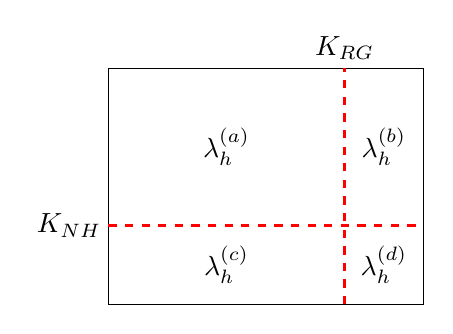
\begin{tikzpicture}
        \draw  (0,0) rectangle (4,3);
        \draw [dashed, red, thick] (0,1) -- (4,1);
        \draw [dashed, red, thick] (3,0) -- (3,3);
        \node at (-.5,1) {$K_{\NH}$};
        \node at (3,3.25) {$K_{\RG}$};
        \node at (1.5,2) {$\lambda_{h}^{(a)}$};
        \node at (3.5,2) {$\lambda_{h}^{(b)}$};
        \node at (1.5,.5) {$\lambda_{h}^{(c)}$};
        \node at (3.5,.5) {$\lambda_{h}^{(d)}$};
    \end{tikzpicture}
\end{center}
\textbf{Lemma.}\\
\begin{itemize}

\item If $\lambda_{\NH}^{(a)}\leq \lambda_{\NH}^{(b)}$ and $\lambda_{\NH}^{(c)}\leq \lambda_{\NH}^{(d)}$ then $f_{\NH}(k)$ is a non-decreasing function in $k$.
\item If $\lambda_{\RG}^{(a)}\leq \lambda_{\RG}^{(c)}$ and $\lambda_{\RG}^{(b)}\leq \lambda_{\RG}^{(d)}$ then $f_{\RG}(k)$ is a non-decreasing function in $k$.

\end{itemize}
}


\frame{
\begin{center}
\includegraphics[width=.8\textwidth]{./Images/proof.pdf}
\end{center}
}

\frame{
$$
\begin{array}{cc}
\includegraphics[width=.5\textwidth]{./Images/best_responses_model1.pdf}&
\includegraphics[width=.5\textwidth]{./Images/best_responses_model1_t=0_6.pdf}\\
\text{($t=0.8$)}&\text{($t=0.6$)}
\end{array}
$$
}

\frame{
\Huge
$$\text{PoA}={{T^*}\over{\widetilde{T}}}$$
}

\frame{
\begin{center}
\includegraphics[width=.8\textwidth]{./Images/model2targetvdemand.pdf}
\end{center}
}

\frame{
\begin{center}
\includegraphics[width=.8\textwidth]{./Images/argminPoAmodel2.pdf}
\end{center}
}

\frame{
\frametitle{Conclusions}
\begin{itemize}
\item Developed a strategic form game representation of CCU interaction;
\item Proved structural properties of equilibrium behaviour;
\item Identified a potential justified approach to obtaining policies.
\end{itemize}
\pause

    \textbf{Measuring the Price of Anarchy in Critical Care Unit Interactions}, \textit{Submitted to OMEGA}

}

\frame{
\begin{center}
\href{https://plus.google.com/+VincentKnight/posts}{+Vincent.Knight}\\
\href{https://twitter.com/drvinceknight}{@drvinceknight}\\
\framebox{\href{http://drvinceknight.github.io/Talks/}{drvinceknight.github.io/Talks}}\\
\vspace{1cm}
\href{https://twitter.com/IzabelaKomenda}{@IzabelaKomenda}\\
Professor Jeff Griffiths
\end{center}
}

\end{document}
